\chapter{Results}
Some of the results in this chapter are based on evaluating the hardware model (HWM) against other models implementing the same neural network. The other models include my software model (SWM), PyTorch running on the CPU (PyCPU), and PyTorch running on the GPU (PyGPU). My software model performs the same computations as the hardware model, so this provides insight to speedup over CPU without computational optimizations. The PyTorch CPU and GPU models then compare my hardware accelerator against heavily-optimized neural network frameworks. A training epoch in the following experiments is defined as performing learning on the 60,000 training images of the MNIST dataset. Inference experiments measure time to perform inference on all 70,000 images in the MNIST dataset.

\todo[inline]{runtime not speedup/eff}
Figures \ref{gpu-speedup} and \ref{gpu-eff} show PyGPU speedup and efficiency for varying batch sizes, respectively. As one might notice, there is no degradation in efficiency whatsoever. In fact, there are efficiencies even higher than 1. For batch size, this is plausible because increasing the batch size will slightly decrease the amount of work needed to be performed. The amount of forward and backward passes remains the same, though only 1 update of the weights needs to be performed for each batch. This means that a batch size of 1 performs 5 times more weight updates than a batch size of 5, which performs 20 times more weight updates than a batch size of 100. Therefore it is for this reason that efficiency remains around 1 even with massive batch sizes. Ultimately, it shows the massive amount of parallelism present in the training of neural networks. 

From the figures, it is clear that the GPU model takes advantage of data-level parallelism to achieve performance, as epoch time is a near linear function of batch size. As a result, since the GPU-based implementation uses a coarser form of parallelism compared to the HWM, it would be illogical to benchmark speedup against the GPU with a batch size of 1. Therefore, the PyGPU model has been benchmarked using a batch size of 50 unless otherwise specified. It should be noted that the PyGPU model also performs 49 fewer weight updates as a result of this. Moreover, each weight update on a GPU would require reductions of partial gradient results from the CUDA kernels, so this should be taken into consideration when observing the following performance benchmarks.

\begin{figure}
	\centering
	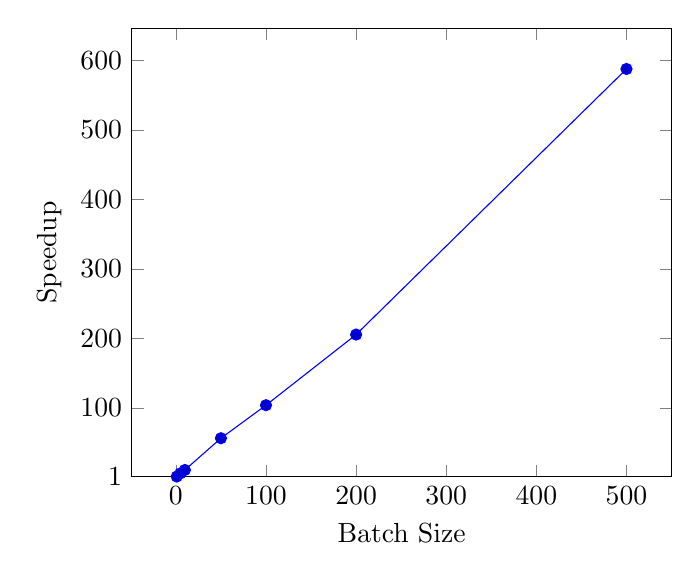
\begin{tikzpicture}
	\begin{axis}
	[ymin=1, ytick = {1, 100, 200, 300, 400, 500, 600}, ylabel={Speedup}, xlabel={Batch Size}]
	\addplot coordinates 
	{(1,1) (5, 5.59) (10, 10.436) (50, 56.178) (100, 103.73) (200, 205.404) (500, 587.764)};
	\end{axis}
	\end{tikzpicture}
	\caption{GPU speedup by increasing batch size}
	\label{gpu-speedup}
\end{figure}

\begin{figure}
	\centering
	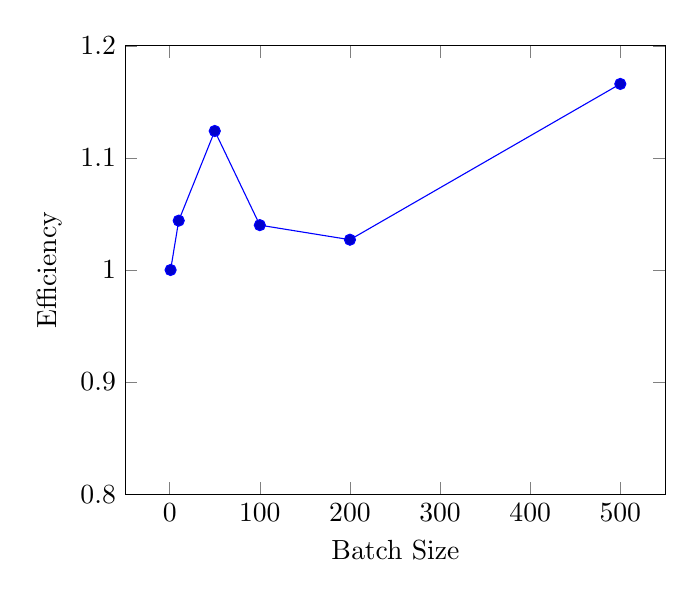
\begin{tikzpicture}
	\begin{axis}[
	ymin=0.8, ymax = 1.2, ylabel={Efficiency}, xlabel={Batch Size}]
	\addplot coordinates 
	{(1,1) (10, 1.044) (50, 1.124) (100, 1.04) (200, 1.027) (500, 1.166)};
	\end{axis}
	\end{tikzpicture}
	\caption{GPU efficiency by increasing batch size}
	\label{gpu-eff}
\end{figure}

\section{Evaluation Hardware}
The hardware model is evaluated using a ZedBoard equipped with a Zynq-7000 XC7Z020 SoC. The SWM and PyCPU both run on a Intel Core i7-4720HQ CPU. The GPU is an Nvidia GeForce GTX 970M equipped with 6 GB of GDDR5 RAM.

\section{Performance}
One of the most important metrics for an accelerator is runtime performance. 
While this hardware model is primarily focused on training, experiments to determine performance for both training and inference modes have both been conducted and are shown in this section.

\subsection{Training}
The average time for 1 training epoch has been recorded for each of the neural network models. The result is shown in Figure \ref{train-runtime-res}. This graph shows that the accelerator massively outperforms CPU models. Figure \ref{train-speedup-res} shows the speedup of the models, using PyCPU as a baseline. Notably, the HWM achieves a speedup of of nearly equal to that of the PyGPU model.

\begin{figure}
	\centering
	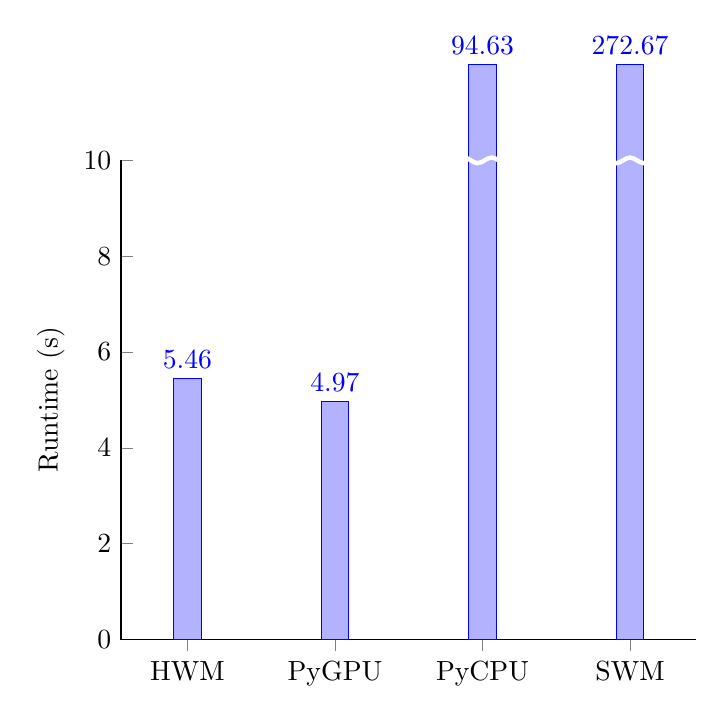
\begin{tikzpicture}
	\begin{axis}[
	ybar,
	width=3.5in,
	enlarge y limits=false,
	enlarge x limits=0.15,
	legend style={at={(0.5,-0.15)},
		anchor=north,legend columns=-1},
	ylabel={Runtime (s)},
	ymin=0,
	ymax=10,
	xmax=SWM,
	restrict y to domain*=0:12, % Cut values off at 14
	visualization depends on=rawy\as\rawy, % Save the unclipped values
	after end axis/.code={ % Draw line indicating break
		\draw [ultra thick, white, decoration={snake, amplitude=1pt}, decorate] (rel axis cs:0.1,1.0) -- (rel axis cs:1.0,1.0);},
	axis lines*=left,
	clip=false,
	nodes near coords={{\pgfmathprintnumber{\rawy}}},
	symbolic x coords={HWM, PyGPU, PyCPU, SWM},
	xtick={data}
	]
	
	\addplot coordinates {(HWM, 5.455)  (PyGPU, 4.9689) (PyCPU, 94.633) (SWM, 272.67)};
	
	\end{axis}
	\end{tikzpicture}
	\caption{Training runtime for various network models}
	\label{train-runtime-res}
\end{figure}

\begin{figure}
	\centering
	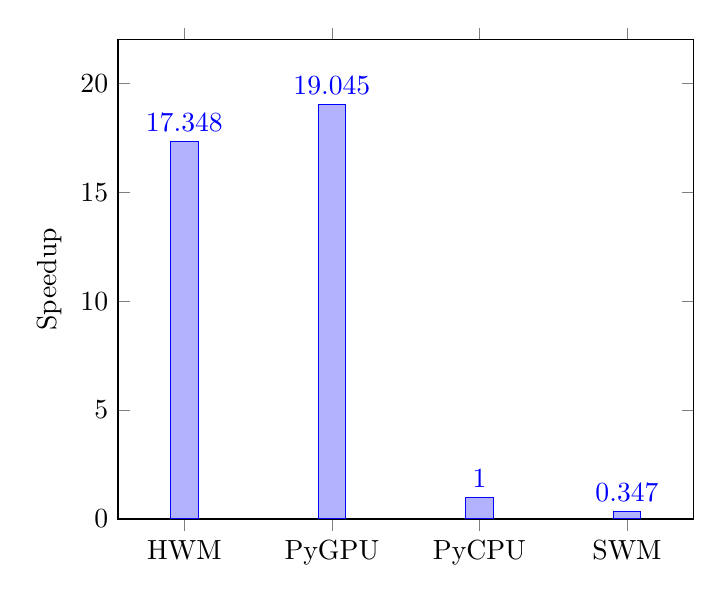
\begin{tikzpicture}
	\begin{axis}[
	ybar,
	width=3.5in,
	enlarge y limits=false,
	enlarge x limits=0.15,
	legend style={at={(0.5,-0.15)},
		anchor=north,legend columns=-1},
	ylabel={Speedup},
	ymin=0,
	ymax=22,
	xmin=HWM,
	xmax=SWM,
	symbolic x coords={HWM, PyGPU, PyCPU, SWM},
	xtick={data},
	scaled y ticks=false,
	nodes near coords,
	nodes near coords style={/pgf/number format/fixed},	
	nodes near coords style={/pgf/number format/precision=3},
	nodes near coords align={vertical}
	]
	
	\addplot coordinates {(HWM, 17.348)  (PyGPU, 19.045) (PyCPU, 1) (SWM, 0.347)};
	
	\end{axis}
	\end{tikzpicture}
	\caption{Training speedup using the PyCPU as a baseline}
	\label{train-speedup-res}
\end{figure}


\subsection{Inference}
Inference performance was also measured for each of the models. The result is shown in Figure \ref{inf-runtime-res}. This graph shows that the accelerator also outperforms CPU models for inference, though falls short of the GPU model. Figure \ref{inf-speedup-res} shows the speedup of the models, using PyCPU as a baseline. The HWM achieves a speedup of 2.282 compared to the PyCPU model.

\begin{figure}
	\centering
	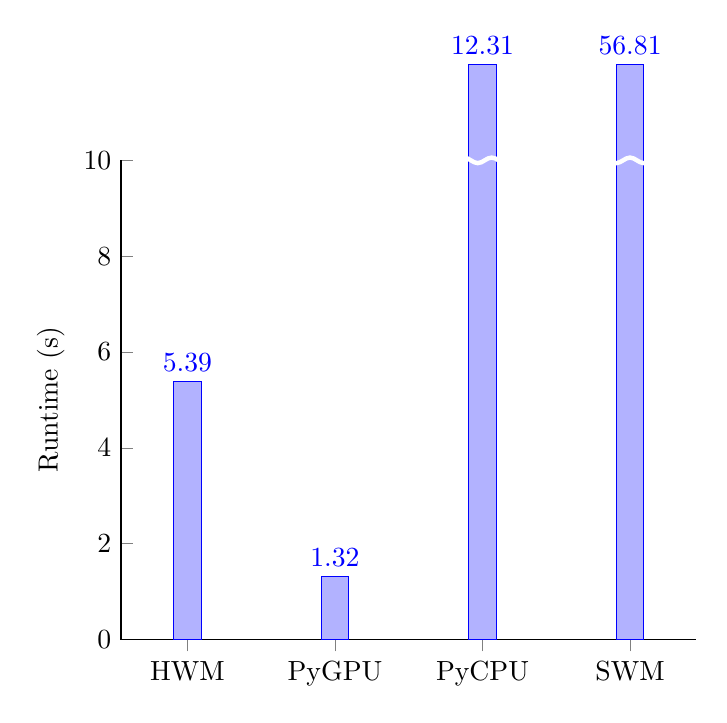
\begin{tikzpicture}
	\begin{axis}[
	ybar,
	width=3.5in,
	enlarge y limits=false,
	enlarge x limits=0.15,
	legend style={at={(0.5,-0.15)},
		anchor=north,legend columns=-1},
	ylabel={Runtime (s)},
	ymin=0,
	ymax=10,
	xmax=SWM,
	restrict y to domain*=0:12, % Cut values off at 14
	visualization depends on=rawy\as\rawy, % Save the unclipped values
	after end axis/.code={ % Draw line indicating break
		\draw [ultra thick, white, decoration={snake, amplitude=1pt}, decorate] (rel axis cs:0.1,1.0) -- (rel axis cs:1.0,1.0);},
	axis lines*=left,
	clip=false,
	symbolic x coords={HWM, PyGPU, PyCPU, SWM}, 
	nodes near coords={{\pgfmathprintnumber{\rawy}}},
	xtick={data}
	]
	
	\addplot 
	coordinates {(HWM, 5.392)  (PyGPU, 1.32) (PyCPU, 12.305) (SWM, 56.808)};
	
	\end{axis}
	\end{tikzpicture}
	\caption{Inference runtime for various network models}
	\label{inf-runtime-res}
\end{figure}

\begin{figure}
	\centering
	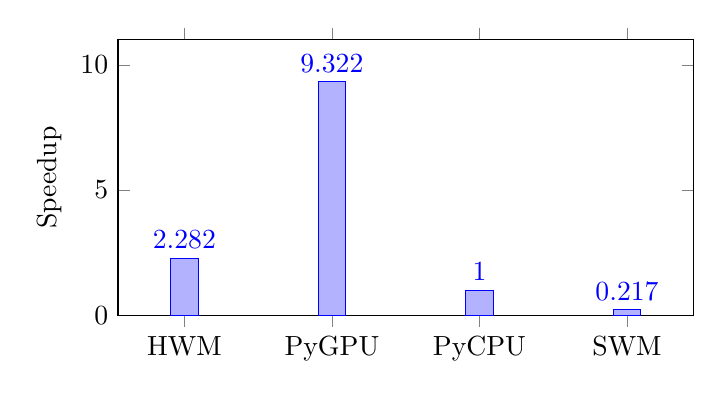
\begin{tikzpicture}
	\begin{axis}[
	ybar,
	height=2in,
	width=3.5in,
	enlarge y limits=false,
	enlarge x limits=0.15,
	legend style={at={(0.5,-0.15)},
		anchor=north,legend columns=-1},
	ylabel={Speedup},
	ymin=0,
	ymax=11,
	xmin=HWM,
	xmax=SWM,
	symbolic x coords={HWM, PyGPU, PyCPU, SWM},
	xtick={data},
	scaled y ticks=false,
	nodes near coords,
	nodes near coords style={/pgf/number format/fixed},	
	nodes near coords style={/pgf/number format/precision=3},
	nodes near coords align={vertical}
	]
	
	\addplot coordinates {(HWM, 2.282)  (PyGPU, 9.322) (PyCPU, 1) (SWM, 0.217)};
	
	\end{axis}
	\end{tikzpicture}
	\caption{Inference speedup using the PyCPU as a baseline}
	\label{inf-speedup-res}
\end{figure}

\subsection{Active/Idle Cycles}
To determine the impact of using MMIO via AXI bus to transfer image data between the PS and the FPGA, active and idle cycles were measured during training and inference. An active cycle is defined as a cycle on the FPGA during which at least one of the layers was computationally active. An idle cycle is thus defined as a non-active cycle. 

An experiment was performed to measure active cycle percentages for the HWM during inference and training. The dataset was the entire MNIST dataset in both cases. The active cycle percentage for inference and training are shown in Table \ref{active-cycle-table}.

\begin{table}
	\centering 
	\begin{tabular}{|c|c|}
		\hline
		& \textbf{Active Cycle Percentage} \\\hline
		Inference & 25.13\% \\\hline 
		Training & 69.20\% \\\hline
	\end{tabular}
	\caption{Active Cycle Percentages for inference and training.}
	\label{active-cycle-table}
\end{table}

This experiment was performed to evaluate if the sending of input over MMIO was the bottleneck of the system. As can be clearly seen from the table, the MMIO transfer of training data was indeed the bottleneck. Furthermore, since backpropagation requires roughly double the amount of work compared to inference, it makes sense that training (which is both inference and backpropagation) is roughly a factor of 3 more active.

\section{Training Accuracy}
This section details the accuracy of the training process using the hardware accelerator. Varying training dataset sizes were chosen during the training process as the reduced precision training resulted in non-convergent training. As such, the training accuracy experiment conducted modified two variables: the learning rate and the training dataset size. 

The tested learning rates were $2^{-7}$, $2^{-8}$, $2^{-9}$, and $2^{-10}$ (0.0078, 0.0039, 0.00195, and 0.000977). This is because the hardware model performs the learning rate multiplication by using bitshifts. The experiments recorded the peak test data set accuracy during the training process. Note that the test dataset size for each run is 70000 minus the size of the training dataset. The results are shown in Figure \ref{training-accuracy}. In this experiment, the highest accuracy, 85.845\%, was achieved with a learning rate of $\eta = 2^{-9}$ and with a dataset of size 4,000.

\begin{figure}
	\centering
	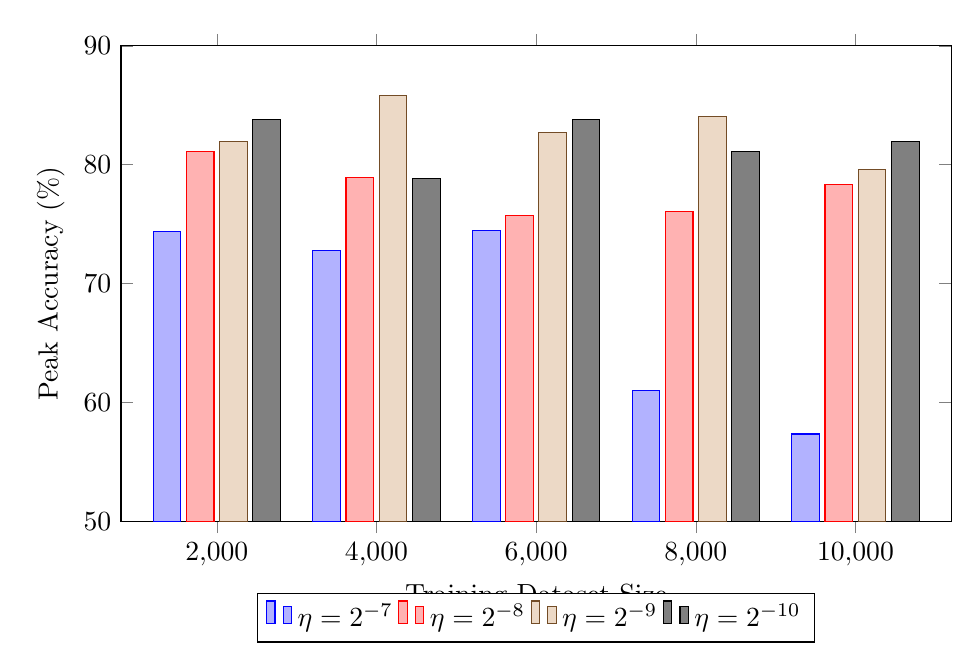
\begin{tikzpicture}
	\begin{axis}[
	ybar,
	height=3in,
	width=\textwidth,
	enlarge y limits=false,
	enlarge x limits=0.15,
	legend style={at={(0.5,-0.15)},
		anchor=north,legend columns=-1},
	ylabel={Peak Accuracy (\%)},
	xlabel={Training Dataset Size},
	ymin=50,
	ymax=90,
	xtick={data},
	scaled y ticks=false,	
	scaled x ticks=false,
	]
	
	\addplot coordinates {(2000, 74.401)  (4000, 72.814) (6000, 74.49) (8000, 61.03) (10000, 57.34)};
	
	\addplot coordinates {(2000, 81.14)  (4000, 78.94) (6000, 75.70) (8000, 76.09) (10000, 78.36)};
	
	\addplot coordinates {(2000, 81.97)  (4000, 85.845) (6000, 82.737) (8000, 84.02) (10000, 79.62)};
	
	\addplot coordinates {(2000, 83.79)  (4000, 78.8) (6000, 83.78) (8000, 81.11) (10000, 81.98)};
	\legend{$\eta = 2^{-7}$, $\eta = 2^{-8}$, $\eta = 2^{-9}$, $\eta = 2^{-10}$}
	\end{axis}
	\end{tikzpicture}
	\caption{Maximum training accuracy reached for various learning rate and training set sizes.}
	\label{training-accuracy}
\end{figure}

\todo[inline]{convergences for swmodel on the network}

\subsection{Stability of Training}
As previously mentioned, due to the relatively low training precision of 18-bit fixed-point, the training process does not converge to a maximum training accuracy, but rather it will reach a maximum training accuracy, and then accuracy will degrade as precision errors accumulate over the training process. Training statistics for the first 10 epochs of the most optimal training configuration from Figure \ref{training-accuracy} illustrate this phenomenon and are shown in Figure \ref{epoch-by-epoch}.

\begin{figure}
	\centering
	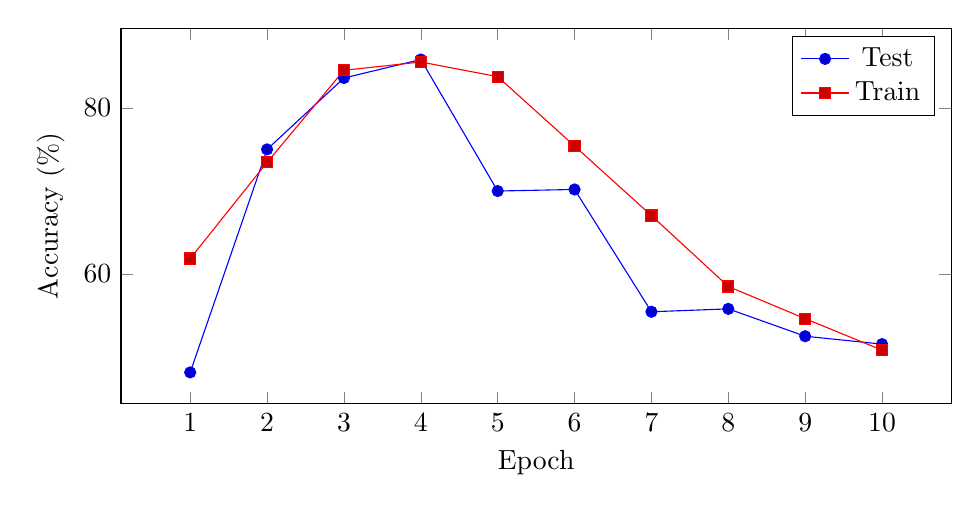
\begin{tikzpicture}
	\begin{axis}[
	ylabel={Accuracy (\%)}, 
	xlabel={Epoch},
	width=\textwidth,
	height=2.5in,
	]
	
	\addplot coordinates 
	{(1, 48.12) (2, 75.012) (3, 83.62) (4, 85.85) (5, 69.99) (6, 70.18) (7, 55.43) (8, 55.78) (9, 52.48) (10, 51.53)};
	\addplot coordinates 	
	{(1, 61.85) (2, 73.45) (3, 84.55) (4, 85.55) (5, 83.78) (6, 75.42) (7, 67.03) (8, 58.48) (9, 54.6) (10, 50.8)};
	
	\legend{Test, Train}
	\end{axis}
	\end{tikzpicture}
	\caption{Epoch-by-epoch training data for an HWM configuration. Clearly visible degradation of accuracy instead of convergence after epoch 4.}
	\label{epoch-by-epoch}
\end{figure}


\section{Implemented Design}
The design implemented for the FPGA is shown in Figure \ref{impl-design}. As expected, the FC1 layer is by and large the most resource intensive, as it utilizes 196 kernels. It is interesting to observe the clustering of individual layer modules, while the interlayer activation buffer for FC0 and FC1 is widely spread out through the FPGA. This would indicate that this interlayer activation buffer was frequently routed to as a midpoint between FC0 and FC1. 

It should be noted that implementation is a non-deterministic process and every design run should result in a slightly different implemented design. However, general trends for routing of the design tend to  persist throughout multiple runs, despite the non-determism of the placing and routing algorithms.

\begin{figure}
	\centering
	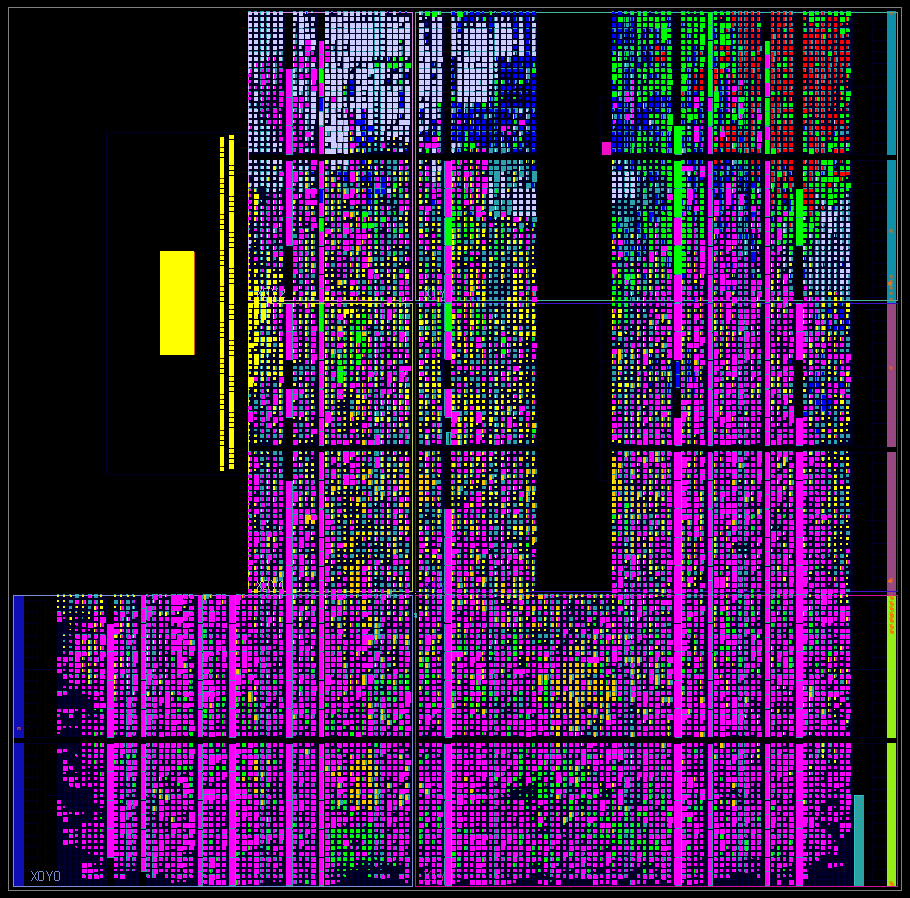
\includegraphics[width=\textwidth]{figures/impl_design}
	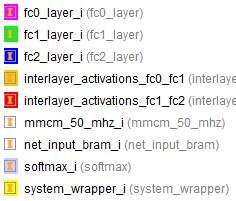
\includegraphics{figures/impl_design_legend}
	\caption{The implemented design of the hardware model}
	\label{impl-design}
\end{figure}

\subsection{Resource Usage, Power, and Timing}
The resource usage of the hardware model is shown in Table \ref{resource-usage}. As can be seen, the DSP slice is the scarcest resource, with LUTs and BRAMs also heavily being used.  Overall, high utilization of the FPGA resources were made to optimize the performance of the accelerator as much as possible.
\begin{table}
	\centering 
	\begin{tabular}{|l|l|l|c|}
	\hline 
	\textbf{Resource} & \textbf{Utilization} & \textbf{Available} & \textbf{Utilization \%} \\\hline 
	LUT & 41132 & 53200 & 77.32		\\\hline
	FF & 54097 & 106400 & 50.84 \\\hline 
	BRAM & 107.5 & 140 & 76.79 \\\hline 
	DSP & 215 & 220 & 97.73 \\\hline	
	\end{tabular}
\caption{Resource usage of the implemented design}
\label{resource-usage}
\end{table}

According to the Vivado report, the total on-chip power of the design is 2.798 Watts. While this number is reported with `Low' confidence by Vivado, this wattage is far lower than typical GPU power consumptions. Power measurements have not been made for the internal GPU during these experiments, though measurements using the Torch framework were made and reported GPU average power at 94.19 Watts while performing training using the AlexNet architecture.The power measurements were performed with an Nvidia Tesla K20M GPU with 5 GB of GDDR5 SDRAM, a top-of-the-line GPU \cite{xinbochen2016}. This is several magnitudes higher than the FPGA based solution in this thesis. 

The implemented design for the hardware model is clocked at a frequency of 50 MHz. Placement and routing are both able to successfully complete with 0 timing violations. There was no need to improve frequency because the current performance bottleneck of this design stems from data transfer over the AXI bus and not from FPGA computational speed.